\documentclass[../../main.tex]{subfiles}

% 

\begin{document}
\chapter{Mössbauerova spektroskopie}

\begin{center}
	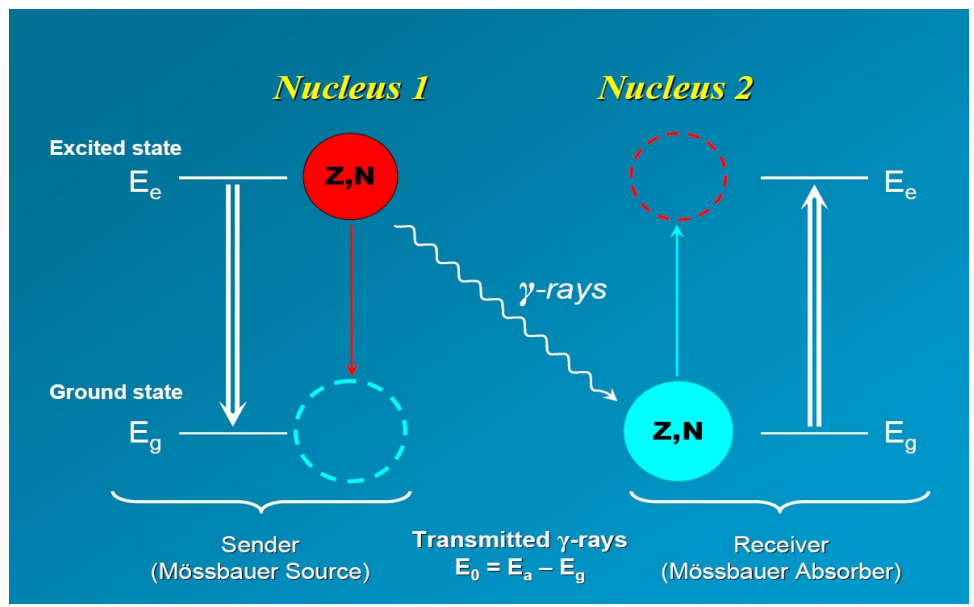
\includegraphics[width=0.7\textwidth]{moss.png}
	\captionof{figure}{Mössbauerova spektroskopie \label{obr:JS7.8}}		
\end{center}

Mössbauerova spektroskopie je založena na tzv. Mössbauerově jevu, který v roce 1958 experimentálně prokázal a teoreticky zdůvodnil R. L. Mössbauer. Za tento objev mu byla udělena Nobelova cena za fyziku v roce 1961. Tato měřicí metoda je založena na jevu bezodrazové rezonanční emise a absorpce záření $\gamma$ v pevných látkách. Má velmi široký potenciál v materiálovém výzkumu, kdy Mössbauerův efekt můžeme pozorovat na více než 20-ti izotopech prvků. Tabulka použitelných prvků je uvedena na Obr.\ref{obr:JS7.1}, z nich je nejčastěji používáno Fe, Sn a Au. Jedná se o prvkově selektivní měřicí metodu, kdy selekce je provedena výběrem zářiče, odpovídajícího pro daný prvek. Nutností je provozovat tuto měřicí metodu v laboratořích schválených státním úřadem pro jadernou bezpečnost (SÚJB). Z naměřených spekter můžeme pomocí jejich vyhodnocení získat parametry hyperjemné struktury vzbuzených stavů sledovaných atomů: izomerní posuv, kvadrupólovou interakci a magnetickou interakci. 


\begin{center}
	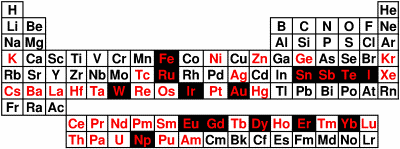
\includegraphics[width=0.9\textwidth]{tabulkaMoess.png}
	\captionof{figure}{Prvky použitelné pro Mössbauerovu spektroskopii (červeně) a nejpoužívanější prvky (s černým pozadím) \label{obr:JS7.1}}		
\end{center}

\begin{itemize}
\item Izomerní posuv, též nazývaný jako chemický posuv, nese informaci o valenčním
stavu sledované komponenty ve spektru a také o jeho spinovém stavu. Změna izomerního posunu je způsobena interakcí elektrického náboje jádra s elektronovými obaly. Ke změně izomerního posuvu dochází také v případě změny teploty vzorku.

\begin{center}
	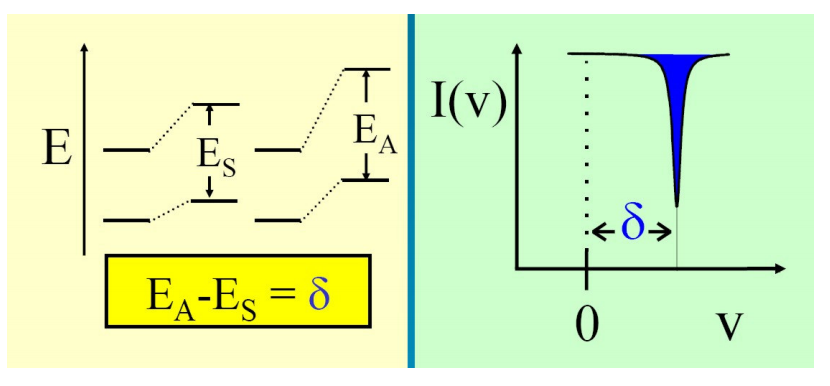
\includegraphics[width=0.7\textwidth]{izomer.png}
	\captionof{figure}{Monopolní interakce – coulombovská interakce mezi protony a $"s"$ elektrony. Stínící efekt d-elektronů: vyšší valence (nižší spinový stav) $\rightarrow$ menší stínění s-elektronů $\rightarrow$ větší elektronová hustota	v oblasti jádra $\rightarrow$ menší izomerní posun $\delta$ \label{obr:JS7.10}}		
\end{center}

\item Kvadrupólová interakce, nese informaci o lokální symetrii okolí sledovaného jádra. Je přímým projevem interakce kvadrupólového momentu jádra a nehomogenního elektrického pole elektronového okolí.

\begin{center}
	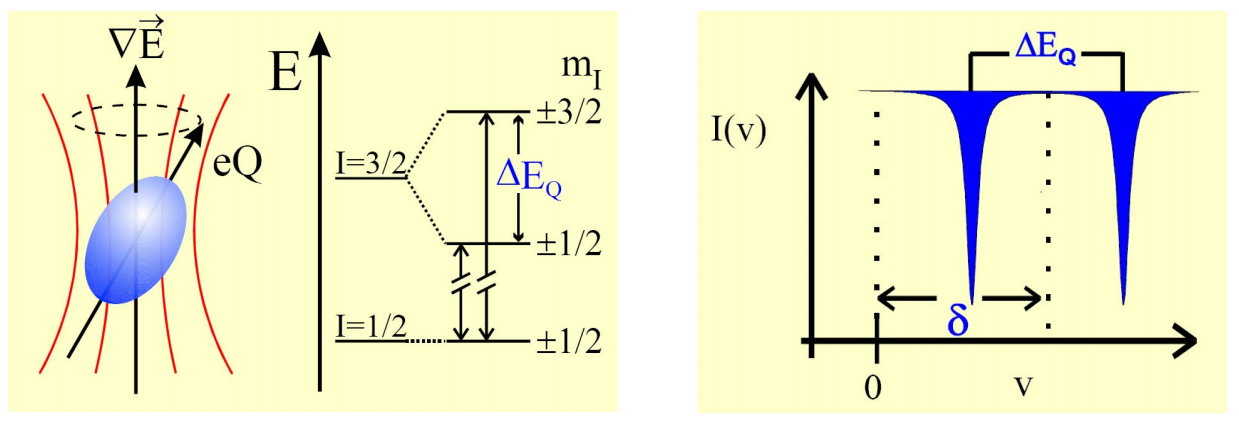
\includegraphics[width=0.9\textwidth]{kvadr.png}
	\captionof{figure}{Kvadrupólová interakce – interakce mezi kvadrupólovým momentem jádra a nehomogenním elektrickým polem $\rightarrow$ kvadrupólové štěpení $\Delta E_Q$ \label{obr:JS7.11}}		
\end{center}

\item Magnetická dipólová interakce, přináší informaci o magnetickém chování studovaného materiálu. Při měření za různých teplot můžeme pozorovat magnetické přechody. Jedná se o interakci mezi magnetickým dipólovým momentem jádra a magnetickým polem.

\begin{center}
	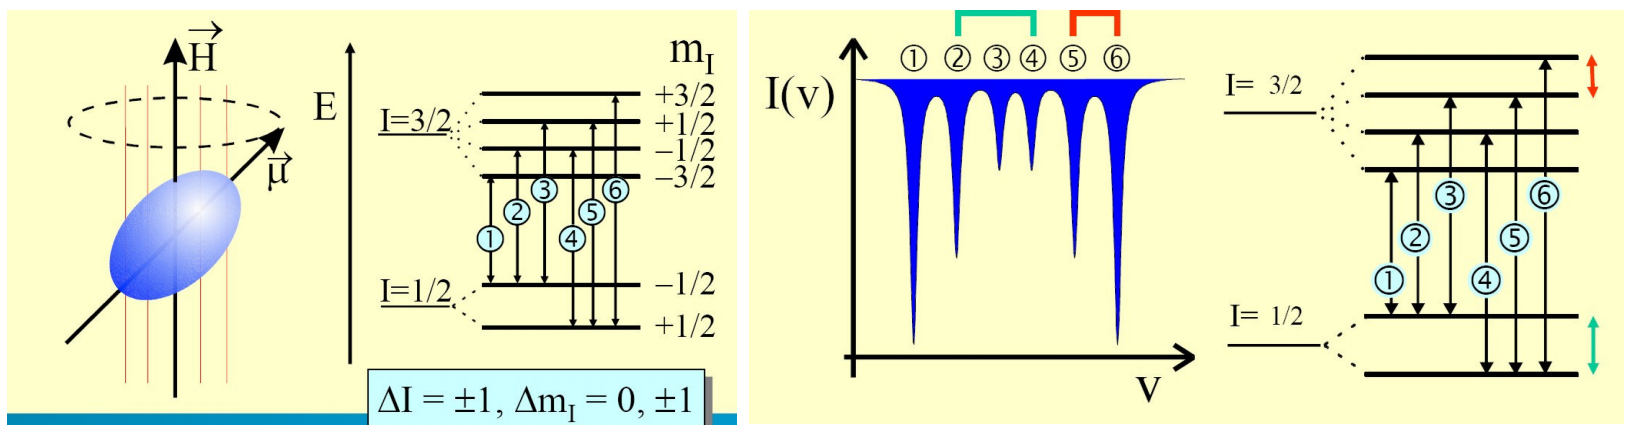
\includegraphics[width=0.9\textwidth]{magnet.png}
	\captionof{figure}{Magnetická dipólová interakce – interakce mezi magnetickým dipólovým momentem
		jádra a magnetickým polem $\rightarrow$ hyperjemné magnetické pole (indukce) $B_{hf}$. Dává nám informace o magnetickém chování a teplotě magnetických přechodů \label{obr:JS7.12}.}		
\end{center}

\end{itemize}

\subsection{Jak eliminovat zpětný ráz?}

\begin{center}
	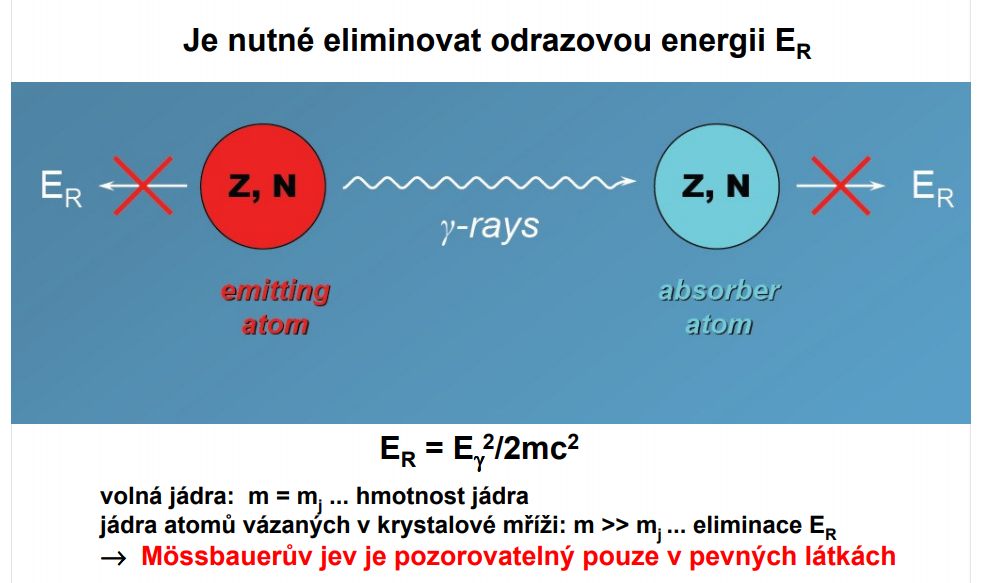
\includegraphics[width=0.9\textwidth]{moss2.png}
	\captionof{figure}{Eliminace odrazové energie $E_R$ \label{obr:JS7.9}}		
\end{center}

Pro atomy vázané v krystalické mřížce je efektivní hmotnost výrazně větší $\rightarrow$ snížení efektu zpětného rázu. Snížením energie $\gamma$-záření lze zredukovat zpětný ráz.  

\section{Mössbauerův jev}

Dříve než přejdeme k výkladu vlastního M$\ddot{O}$SSBAUEROVA efektu, je třeba se krátce zmínit o takzvané jaderné fluorescenci, jejíž pozorování s Mössbauerovým objevem těsně souvisí. Podobně jako v elektronovém obalu atomu i v jádru může dojít k rezonanční absorpci kvanta $\gamma$, jehož energie odpovídá přesně energetickému rozdílu výchozího a konečného stavu jádra. Pozorování této jaderné fluorescence pomocí
kvant $\gamma$ emitovaných jádry je ztíženo tím, že tato kvanta nemají již rezonanční energii, protože část energie přechodu přejde v kinetickou energii zpětného odrazu jádra. K vyvolání jaderné fluorescence je naopak třeba kvant s energií větší, než odpovídá přechodu, protože část energie při absorpci se opět projeví
jako kinetická energie vzbuzeného jádra, kterým byl foton absorbován. Pomocí Dopplerova efektu lze principiálně dosáhnout zvětšení energie emitovaného fotonu tím, že foton je vyslán jádrem pohybujícím se směrem k absorbujícímu rychlostí $v$. Změna frekvence je dána známým vztahem
\begin{equation}
\Delta \nu = \nu \dfrac{v}{c},
\end{equation}
kde $\nu$ je frekvence fotonu a $c$ je rychlost světla.

Energie odrazu $R = E^2 /2 M c^2$, kde $E$ je energie fotonu a $Mc^2$ je klidová energie jádra. Klidové energie u středně těžkých jader jsou řádově $10^{11} ~\mathrm{eV}$, takže při energii kvanta $\gamma$ rovné $10^{6} ~\mathrm{eV}$ činí energie zpětného odrazu $5 ~\mathrm{eV}$. K vykompenzování ztrát energie jak při emisi tak i při absorpci je třeba udělit emitujícímu jádru rychlost přibližně $3 \cdotp 10^5 ~\mathrm{cm/s}$. Dalším faktorem důležitým pro pozorování jaderné fluorescence je monochromatičnost
kvant $\gamma$. Šířky rezonančních a absorpčních linií jsou dány vztahem
\begin{equation}
\Gamma = \dfrac{\hbar}{\tau},
\end{equation}
kde $\hbar$ je redukovaná Planckova konstanta a $\tau$ je střední doba života vzbuzeného stavu. Při $\tau = 10^{-10} ~\mathrm{s}$ je šířka linie přibližně $6 \cdotp 10^{-6} ~\mathrm{eV}$. Natolik monochromatická
musí být kvanta $\gamma$, aby se jaderná fluorescence výrazně projevila. Je zřejmé, že tepelný pohyb jader způsobí polychromatičnost o několik řádů větší, než je šířka emisní nebo absorpční linie. Veliký účinný průřez pro rezonanční absorpci umožňuje však na druhé straně její pozorování i v případě, jestliže jen
malá část kvant $\gamma$ splňuje rezonanční podmínky. Je samozřejmé, že rezonanční absorpce je lépe pozorovatelná na jádrech s malou střední dobou života, která mají širokou rezonanční linii. 

Při pokusech s jadernou fluorescencí bylo zvoleno k dosažení potřebné rychlosti emitujícího jádra několik způsobů. Látka obsahující radioaktivní jádra byla zahřívána na vysokou teplotu, a tím se objevila grupa jader majících postačující rychlost. Bylo rovněž použito centrifugy s vysokou obvodovou rychlostí, na jejímž obvodu byla nanesena radioaktivní jádra. Třetí cesta záležela konečně na tom, že jádro emitovalo ještě během pohybu, v kterém se nacházelo v důsledku zpětného odrazu při emisi částice, která předcházela
emisi $\gamma$. Vhodnou volbou úhlu mezi směrem emise této částice a směrem letu následujícího kvanta $\gamma$ lze vybrat rychlost jádra potřebnou k vyvolání žádoucího Dopplerova posuvu. Žádnou z uvedených metod nelze získat zcela monochromatické záření $\gamma$ a pozorovaná jaderná fluorescence leží vždy na hranici pozorovatelských možností. 

V roce 1958 R. M$\ddot{O}$SSBAUER, vycházeje ze známé LAMBOVY teorie o vlivu vazby jádra v krystalové mříži na rozptyl neutronů a ukázal, že za jistých podmínek není jádro vázané v krystalové mříži schopno převzít odrazovou energii při emisi kvanta $\gamma$. Zpětný odraz v tomto případě přejímá celý krystal sestávající z velkého počtu atomů. 

Místo klidové energie jádra ve vztahu pro energii odrazu se objeví klidová energie krystalu, která je o mnoho řádů větší, takže odrazová energie je prakticky nulová a emitované kvantum $\gamma$ je rezonanční. Totéž platí i o absorpci v jádru zabudovaném do podobného krystalu. 

Intenzita rezonančního záření $\gamma$ souvisí s teplotou krystalu $T$ vztahem 
\begin{equation}\label{eq:JS7.1}
I = \exp (-2W(T,R, \Theta)),
\end{equation}
kde 
\begin{equation}\label{eq:JS7.2}
W = \dfrac{3R}{k \Theta} \left[ \dfrac{1}{4} + \left( \dfrac{T}{\Theta} \right)^2 \int_{0}^{\Theta /T} \left( \dfrac{t}{\exp(t) - 1}\right) dt \right] 
\end{equation}
závisí především na poměru energie odrazu $R$ k energii $k \Theta$, odpovídající takzvané DEBYEOVĚ teplotě $\Theta$, a dále na poměru teploty krystalu $T$ k $\Theta$. Při tom $R$ je energie odrazu, kterou by přejalo jádro nevázané v krystalové mříži. Z Debyeova modelu krystalu je třeba připomenout, že $k \Theta $ odpovídá maximální energii ve spektru vlastních kmitů atomů v krystalové mříži. Aby intenzita rezonančního záření byla znatelně různá od nuly, je třeba především, aby $W$ bylo řádově rovno $1$ nebo menší. Minimální hodnota, které $W$ může nabýt bez ohledu na druhý člen v závorce, závisí jen na energii odrazu a na Debyeově
teplotě. Intenzita bude tím větší, čím menší bude odrazová energie a čím vyšší bude Debyeova teplota. Prakticky je proto Mössbauerův efekt omezen na středně těžká až těžká jádra a na energie záření $\gamma$ pod $100 ~\mathrm{keV}$. Druhý člen v závorce ve výrazu pro $W$ závisí na poměru skutečné teploty krystalu k Debyeově a s klesající teplotou $T$ se zmenšuje. Aby nepřispíval k $W$, je třeba pracovat při teplotách $T < 0$.

Vztahy (\ref{eq:JS7.1}) a (\ref{eq:JS7.2}) se zcela shodují s tak zvaným DEBYEOVÝM-WALLEROVÝM faktorem udávajícím intenzitu záření X koherentně rozptýleného na krystalu. Abychom ze vztahů (\ref{eq:JS7.1}) a (\ref{eq:JS7.2}) dostali tento faktor, stačí za odrazovou energii $R$ dosadit energii $E_R$, kterou by ztratil foton záření X při rozptylu na atomu s hmotou $M$ pod úhlem $\vartheta$
\begin{equation}
E_R = \dfrac{E^2}{Mc^2} (1 - \cos \vartheta).
\end{equation}

Maximální $E_R$ je pro $\vartheta =$ $90^{\circ}$ , kdy foton mění svůj impuls ze záporné hodnoty v kladnou. Odrazová energie, kterou v tomto případě přijme atom, je právě rovna dvojnásobku energie odrazu, kterou přejme jádro při emisi stejně energetického kvanta $\gamma$, jehož impuls se mění od nuly před emisí do maximální hodnoty po emisi. Vidíme, že shoda je úplná; jde tedy v podstatě o jeden a tentýž jev, jehož příčinou je vazba atomů, a tedy i jader v krystalové mříži, a jehož důsledkem je neschopnost jednoho jádra nebo atomu převzít energii odrazu ať už koherentně rozptýleného záření X dopadajícího na atom z vnějšku nebo kvanta $\gamma$ emitovaného jádrem.

Pro kvanta $\gamma$ emitovaná v důsledku Mössbauerova jevu bez odrazu atomového jádra se vžilo pojmenování Mössbauerova kvanta $\gamma$, Mössbauerovo záření nebo Mössbauerova linie. Mössbauer odvodil svůj vztah pro intenzitu Mössbauerovy linie pomocí Debyeova modelu krystalu. F. L. ŠAPIRO dospěl k výrazu pro intenzitu Mössbauerovy linie klasickou metodou používanou v teorii frekvenční modulace. Kvantum $\gamma$ emitované jádrem kmitajícím frekvencí $\omega$ je frekvenčně modulované, to jest vedle hlavní nosné frekvence se vytvářejí postranní pásma. Pro intenzitu nosné frekvence vychází Šapirovi vztah
\begin{equation}\label{eq:JS7.3}
I = \exp (- \dfrac{\bar{x}^2}{\lambdabar}),
\end{equation}
v kterém $\bar{x}^2$ je střední kvadratická odchylka atomu v krystalové mříži v důsledku tepelných kmitů,
\begin{equation}
 \bar{x}^2 = \dfrac{1}{n} \sum_n x_{n}^{2},
\end{equation}
$\lambdabar$ je vlnová délka fotonu dělaná $2 \pi$. Tento vztah ukazuje, že intenzita Mössbauerovy
linie bude výrazná tehdy, jestliže střední kvadratická odchylka atomu ze střední polohy bude rovna přibližně vlnové délce fotonu nebo bude menší. Vyjádří-li se střední kvadratická odchylka ve výrazu (\ref{eq:JS7.3}) klasickým způsobem pomocí střední energie oscilátoru a použije-li se Debyeova modelu pro spektrum vlastních kmitů krystalu, dostane se opět původní Mössbauerův vztah.

Podrobnější teorie Mössbauerova efektu byla podána W. M. VISSCHEREM, který ukázal, že při emisi kvanta $\gamma$ jádrem je nejpravděpodobnější vznik nebo zánik pouze jediného fononu\footnote{Fonon je tzv. kvazičástice (nejde tedy o skutečnou částici) šířící vibrační kvantum v krystalové mřížce. Vibrace v krystalové mřížce se mohou přenášet od buňky k buňce a vytvářet tím dojem pohyblivé částice. Tato „částice“ se pak nazývá fonon. Pomocí fononů se popisuje šíření zvuku (zvukových vln) v krystalech.} v krystalové mříži. Současný vznik nebo zánik více fononů je mnohem méně pravděpodobný. Jestliže fononové spektrum krystalu je omezeno snížením teploty hluboko pod Debyeovu na velmi málo energetické fonony, může kvantum $\gamma$ při emisi ztratit nebo získat jen zcela nepatrnou energii a zůstane rezonančním.

Ze všech případů uvedených v tabulce je Mössbauerův efekt nejsnáze pozorovatelný u $^{57}Fe$, a to nejenom proto, že lze pracovat při pokojové teplotě, ale zejména také z toho důvodu, že v místě rezonance klesne intenzita záření za absorbátorem o několik procent, použije-li se železa s přirozeným obsahem $^{57}Fe$ jako absorbátorů a o několik desítek procent při použití absorbátorů obohaceného izotopem $^{57}Fe$. Absorpční spektrum je velmi výrazné a lze na něm studovat velmi jemné efekty.

\section{Použití Mössbauerova jevu}

\subsection{Magnetické pole v místě jádra}

Již v prvních pracích s tímto radioizotopem bylo možno nalézt hyperjemnou strukturu linie $\gamma$ způsobenou rozštěpením vzbuzeného i základního stavu $^{57}Fe$ v magnetickém poli, které u železa ve feromagnetickém stavu v místě jádra existuje.

Stanovení velikosti magnetického pole v místě jádra železa a zejména určení jeho směru má velký význam pro teorii vnitřního magnetického pole. 

\begin{center}
	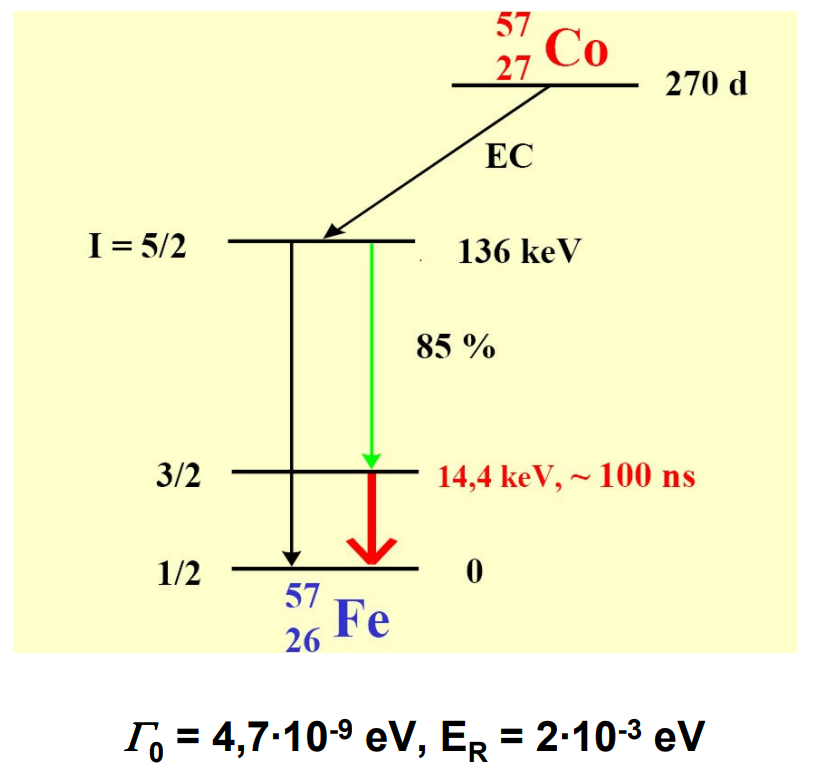
\includegraphics[width=0.6\textwidth]{zelezo.png}
	\captionof{figure}{Rozpadové schéma izotopu $^{57}Fe$ \label{obr:JS7.5}}		
\end{center}

\begin{center}
	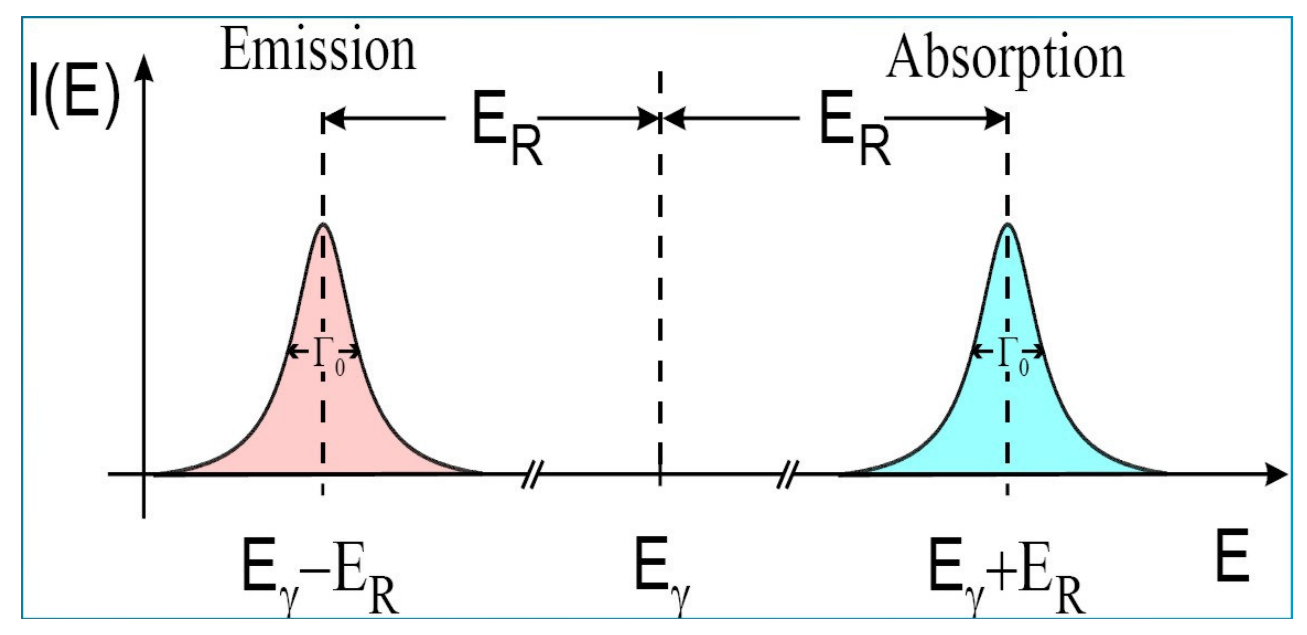
\includegraphics[width=0.7\textwidth]{zelezo2.png}
	\captionof{figure}{ $^{57}Fe$ Mössbauerova spektroskopie, $\Gamma_0 = 4,7 \cdotp 10^{-9} ~\mathrm{eV}, E_R = 2 \cdotp 10^{-3} ~\mathrm{eV}$ \label{obr:JS7.6}}		
\end{center}

\section{Elektrické pole v krystalu}

Malá relativní šířka linie $^{57}Fe$ umožňuje studovat i jemnější efekty způsobené kvadrupólovou interakcí elektrického pole jádra s elektrickým polem uvnitř krystalu. K tomuto účelu je výhodné mít k dispozici zdroj, který nejeví rozštěpení linií. Takový zdroj lze připravit zabudováním atomů $^{57}Co$ do mřížky
nemagnetické oceli. Experimentálně bylo potvrzeno, že v tomto případě skutečně linie zůstává nerozštěpená a její šířka je velmi přesně rovna vlastní šířce.

Pomocí tohoto zdroje sledovali O. C. KISTNER a A. W. SUNYAR u $Fe_2 O_3$ velikost kvadrupólové elektrické interakce, která způsobuje posuvy hladin rozštěpených dříve uvedenou magnetickou interakcí. K posunu, jehož velikost je dána vztahem
\begin{equation}
\epsilon = \dfrac{e^2 q Q}{4I (2I - 1)} [3 m^2 - I(I+1)],
\end{equation}
kde $Q$ je kvadrupólový moment jádra, $I$ je celkový spin jádra, $m$ je magnetické kvantové číslo a $q$ závisí na gradientu intenzity elektrického pole, dochází pouze u vzbuzeného stavu se spinem $3/2$, a to tak, že hladiny s $m = \pm 3/2$ jsou posunuty jedním směrem, hladiny s $m = \pm 1/2$ druhým směrem. Obecně nebývají posuvy způsobené kvadrupólovou interakcí stejně veliké pro všechna $m$. V daném případě je lze však považovat za stejné, protože $\epsilon$ je mnohem menší než rozštěpení způsobené magnetickou interakcí.


\begin{center}
	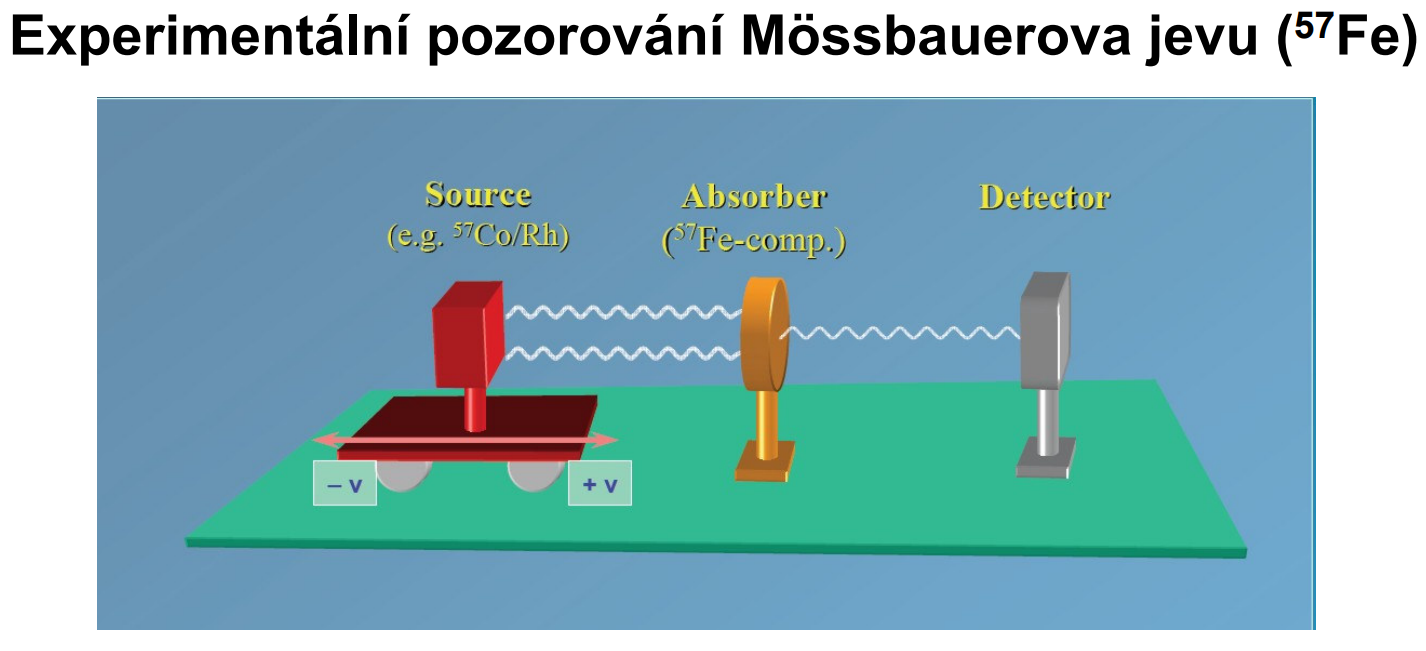
\includegraphics[width=1\textwidth]{zelezo3.png}
	\captionof{figure}{ Hyperjemné elektromagnetické interakce $\rightarrow$ posunutí, rozštěpení hladin energie v jádře, Dopplerovská modulace energie fotonu $\Delta E = E_{\gamma} (\nu /c)$ \label{obr:JS7.7}}		
\end{center}

\section{Dopplerův efekt druhého řádu}

Při experimentech s $^{57}Fe$ se poměrně brzy shledalo, že vedle efektu chemické vazby (izomerického efektu) může dojít k posuvu rezonanční linie z mnoha jiných příčin. Všechny mají svůj původ ve změně fononového spektra krystalu, a tím spojené změny střední hodnoty kvadrátu rychlosti jádra emitujícího
nebo absorbujícího. Jednou z těchto příčin je Dopplerův efekt druhého řádu, který vždy vede ke snížení energie kvanta $\gamma$ a zvýšení střední energie krystalu. Je vyvolán změnou hmoty jádra při emisi nebo absorpci kvanta $\gamma$.


\section{Experimentální uspořádání Mössbauerova spektrometru}

V Mössbauerově spektroskopii existuje velká řada možných experimentálních uspořádání tzv. Mössbauerova spektrometru (MS). Tato uspořádání se liší v rozložení čtyř základních komponent, pohybového zařízení, zářiče, absorbéru (vzorek) a detektoru (případně detekční soustavy). Nejčastěji používané uspořádání je v transmisním módu. Transmisní uspořádání je schematicky znázorněno na Obr.\ref{obr:JS7.2}. Pro měření spekter je nutné doplnit systém o elektroniku pro řízení pohybu a zpracování signálů.

\begin{center}
	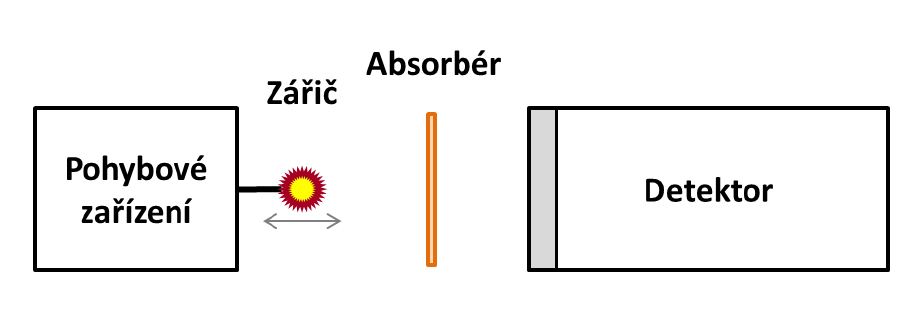
\includegraphics[width=0.9\textwidth]{spektrometr.png}
	\captionof{figure}{Blokové schéma transmisního M$\ddot{o}$ssbauerova spektrometru \label{obr:JS7.2}}		
\end{center}

V transmisním typu geometrického uspořádání MS je možné sestavu snadno modifikovat pro jiné typy měření. Modifikace se provádí upnutím absorbéru (vzorku) do různých komor pro udržení konkrétních nastavených a sledovaných podmínek. Mezi tyto podmínky patří teplota, externí magnetické pole, průtok plynu, tlak atd. Z experimentálního hlediska je velmi zajímavé působit na vzorek pomocí teploty. Pro měření při vysokých teplotách (nad $300 ~\mathrm{K}$) se používají vysokoteplotní pícky. Vysokoteplotní měření umožňují sledovat materiálové transformace, ke kterým dochází za určitých teplot. Tato měření jsou často prováděna s konkrétní atmosférou (např. oxidační nebo redukční). Experimenty mohou být prováděny i při kontrolované vlhkosti.

Pro měření za nízkých teplot se používá různých druhů kryostatů, které se obecně dělí na dva základní druhy a to podle způsobu dosažení nízké teploty. Prvním typem je kryostat s uzavřeným cyklem, kde je pomocí opakované změny tlaku odváděno teplo z prostoru chlazeného vzorku. Tento typ konstrukce se vyznačuje snadným
nastavením různých teplot a nízkými nároky na obsluhu. Nevýhodou u těchto zařízení je přenos vibrací z uzavřeného cyklu na studovaný vzorek. Přenesené vibrace mohou nežádoucím způsobem ovlivnit měřené m$\ddot{o}$ssbauerovské spektrum, způsobují ve sledovaných spektrech rozšíření spektrálních čar. Druhým typem je kryostat plněný kryokapalinami, kdy je k chlazení použit kapalný dusík (teplota $77,4 ~\mathrm{K}$) nebo kapalné hélium (teplota $4,2 ~\mathrm{K}$). U tohoto typu kryostatů jsou vibrace minimální. Hlavní nevýhodou je náročnost na obsluhu těchto zařízení (nutnost pravidelného zajištění, udržování a plnění kryokapalin). U heliových kryostatů jsou také vysoké pořizovací nároky na kapalné helium a jsou zde vyšší nároky na vakuovou izolaci kryostatu. Naproti tomu kryostaty plněné kapalným dusíkem jsou z hlediska provozních nákladů poměrně nenáročné. Chlazení dusíkem je možné provádět pomocí dusíkových par, nebo pomocí teplo vodivého trnu, který propojí vzorek a kapalný dusík. Blokové schéma kryostatu plněného kapalným dusíkem s transmisním M$\ddot{o}$ssbauerovým spektrometrem je na Obr.\ref{obr:JS7.3}.

\begin{center}
	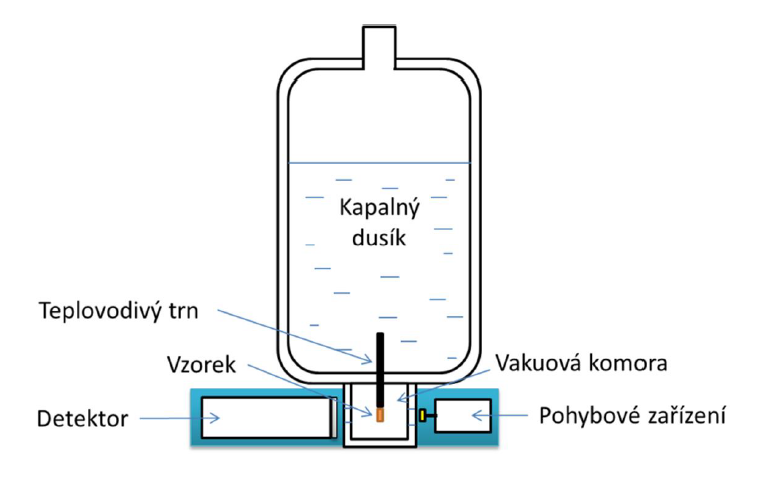
\includegraphics[width=0.9\textwidth]{kryostat.png}
	\captionof{figure}{Blokové schéma kryostatu plněného kapalným dusíkem s transmisn M$\ddot{o}$ssbauerovým spektrometrem \label{obr:JS7.3}}		
\end{center}

\section{Části Mössbauerova spektrometru}

Už bylo řečeno, že nedílnou součástí každého spektrometru jsou pohybové zařízení, zářič, absorbér a detekční soustava. Tyto čtyři hlavní součásti mohou být různě uspořádány. Uspořádání je odvozeno od typu vzorku a vlastností, které na něm chceme studovat. Nedokonalost, nebo nevhodné nastavení těchto klíčových komponent, se vždy projeví negativně v kvalitě naměřeného spektra.

\subsection{Pohybové zařízení}

Pro MS je nutné modulovat energii gama fotonů, čehož je dosaženo pomocí Dopplerova jevu. Pohybové zařízení je tedy využíváno pro modulaci energie vyzařovaných $\gamma$-fotonů ze zářiče. Principiálně je nutné zajistit pohyb zářiče vůči absorbéru. Je tedy možné kmitat jen absorbérem a zářič nechat ve stabilní poloze. Při použití tzv. rezonančního detektoru může být pohybováno jak zářičem, tak detektorem pro dosažení zúžení spektrálních čar. Pro generování pohybu je možné použít dva základní režimy.

\begin{itemize}
	\item KONSTANTNÍ RYCHLOST je používána v průmyslových aplikacích, kde jsou požadavky na měření převážně ve formě porovnání poměru dvou spektrálních komponent. Při měření není snahou vykreslit celé spektrum, ale pouze se zaměřit na zajímavé oblasti. Pro správnou aplikaci je však nutné nejprve změřit celé spektrum a následně je možné se zaměřit na zajímavé body. Následná měření (při konstantní rychlosti) pouze v určitých bodech jsou mnohonásobně rychlejší. 
	
	\item KONSTANTNÍ ZRYCHLENÍ je využíváno v laboratořích jak na zcela neznámých vzorcích
	tak i na známých vzorcích. V tomto měřicím režimu dochází k čítání a vykreslení celého spektra, což zvyšuje délku měření (oproti režimu konstantní rychlosti). Výhodou je možnost vidět celé spektrum, včetně případných postranních komponent a také jeho statistickou kvalitu. 

\end{itemize}

Pro samotnou konstrukci pohybového zařízení je nejčastěji využíváno elektrodynamického principu. Konstrukce se skládá z permanentních magnetů a cívek. K pohybu je využito napětí, které je na cívky přiváděno a následně pomocí cívek je i sledováno pro kontrolu pohybu zpětnou vazbou. 

Další z možností dosažení pohybu je pomocí deformace piezo-krystalů. V těchto případech bývá zářič napařen přímo na piezokrystalu. Výhodou tohoto typu řešení je malý rozměr, možnost pracovat i za nízkých teplot a
případně i v externím magnetickém poli. 

\subsection{Zářič a absorbér}

Z hlediska měření může být studován buď neznámý zářič, nebo neznámý absorbér. Nejčastější použití v materiálovém výzkumu je studium neznámého absorbéru za použití známého zářiče. Pro tyto účely se používá známý zářič s jednou spektrální čárou. Studovaný absorbér může být v různém stavu (například: prášek, tenký film, zmražený roztok, blok materiálu, atd.). V případě studia zářiče se jedná o metodu nazývanou Emisní Mössbauerova spektrometrie (EMS). Pro toto měření je nutné studovaný materiál obohatit radioaktivním izotopem, který přejde radioaktivní přeměnou na jádro studovaného atomu. Pro tyto vzorky je jako absorbér používán materiál, který má jedinou spektrální komponentu a tou je singlet. Absorbér bývá pro tyto účely optimalizován z hlediska obohacení a tloušťky, aby šířka jeho spektrální čáry byla co nejužší a efekt měření byl co největší. Například se používá materiál $K_2 Mg Fe(CN)_6$.


\subsection{Detekční soustava}

Detekce v Mössbauerově spektrometrii je velmi náročná, jelikož detekované $\gamma$ fotony mají z energetického hlediska nízkou úroveň $14,4 ~\mathrm{keV}$. Zároveň dochází ze zdroje k emisi $\gamma$ fotonů s vyšší energií $122,1 ~\mathrm{keV}$, které mohou detektor saturovat. Pro detekci se používá několik typů detektorů, založených na různých principech, kdy se pro jejich správnou funkci vyžadují obvykle napájení vysokým napětím a následné zpracování a zesílení výstupních signálů pomocí předzesilovače a zesilovače.

\begin{itemize}
	\item PROPORCIONÁLNÍ DETEKTORY (plynové) - využívají vlastnosti ionizujícího záření, kdy
	v detektoru dochází k ionizaci plynové náplně. Ionizovaný plyn zprostředkuje vodivé propojení katody a anody. Na výstupu detektoru pozorujeme proudové impulzy. Tyto detektory dosahují velmi kvalitního energetického rozlišení a také vynikají z hlediska linearity. Je možné je použít v experimentech v externím magnetickém poli, bez nutnosti toto pole stínit. Jejich hlavní nevýhodou je stárnutí plynové náplně, relativně nízká detekční účinnost a také relativně velká mrtvá doba, což se u vyšších aktivit zářiče může projevit velmi negativně. Tento typ detektoru bývá v MS nejčastěji používán u experimentů v externím magnetickém poli, protože nevyžaduje stínění.
	\item POLOVODIČOVÉ DETEKTORY - pracují na principu, kdy dopadající $\gamma$ fotony vytvoří páry elektronů a děr, které zprostředkují průchod proudu polovodičem. Tyto detektory dosahují vysokého energetického rozlišení. Mezi jejich nevýhody patří nezbytnost chlazení pro eliminaci tepelného šumu.
	\item SCINTILAČNÍ DETEKTORY - jsou nejpreferovanější možností pro MS. Využívají scintilační krystaly, které převádí $\gamma$ fotony na záblesky fotonů ve viditelné oblasti spektra pomocí luminiscence. Následně jsou záblesky fotonů detekovány pomocí fotonásobiče. Ve srovnání s ostatními typy detektorů mají nižší energetické rozlišení. Pro jejich využití v oblasti $14,4 ~\mathrm{keV}$ je nutná výroba velmi tenkých scintilačních krystalů, což je technologicky náročné. Snížením tloušťky je také snížen vliv $\gamma$ fotonů o energii $122,1 ~\mathrm{keV}$, které jsou ${57}^Co$ emitovány při přechodu ze druhé na první excitovanou hladinu. Jejich hlavní výhodou je dlouhodobá stabilita (i když některé typy scintilačních krystalů mohou časem degradovat). Nevýhodou je, že není možné tyto detektory použít při experimentech v externím magnetickém poli v závislosti na fyzikálním principu fotonásobiče. 
\end{itemize}

\section{Shrnutí}

Z uvedeného přehledu je zřejmé, že Mössbauerův efekt se uplatňuje v mnoha fyzikálních oborech. Absorpční spektrometrie rozvinutá na základě Mössbauerova efektu byla původně určena pro vlastní jadernou fyziku ke studiu hyperjemné struktury vzbuzených stavů. Z přehledu je však zřejmé, že velmi brzy dala neobyčejně závažné informace o vnitroatomárních magnetických polích. Je do jisté míry překvapením, že dává informace o elektrických polích v krystalu a jejich interakcích s jádry, že s její pomocí byly řešeny problémy z oblasti teorie relativity a gravitace, problémy krystalové fyziky a mnohé další otázky. 

\end{document}